\documentclass[conference]{IEEEtran}
\IEEEoverridecommandlockouts
\usepackage{cite}
\usepackage{amsmath,amssymb,amsfonts}
\usepackage{graphicx}
\usepackage{textcomp}
\usepackage{hyperref}
\usepackage{xcolor}
\usepackage{booktabs}
\usepackage{multirow}
\usepackage{placeins}
\usepackage{float}
\usepackage{tikz}
\usetikzlibrary{arrows.meta,backgrounds,fit,positioning,shapes.geometric}

\begin{document}
	
	\title{Towards Practical On-Device Android Malware Detection via Lightweight Static Analysis}
	
	\author{\IEEEauthorblockN{Jarin Tasnim}
		\IEEEauthorblockA{\textit{Department of CSE,}
			\textit{BUET}\\
			2005083@ugrad.cse.buet.ac.bd}
		\and
		\IEEEauthorblockN{Abdullah Faiyaz}
		\IEEEauthorblockA{\textit{Department of CSE,}
			\textit{BUET}\\
			2005065@ugrad.cse.buet.ac.bd}
		\and
		\IEEEauthorblockN{Mohammad Sadnam Faiyaz}
		\IEEEauthorblockA{\textit{Department of CSE,}
			\textit{BUET}\\
			2005111@ugrad.cse.buet.ac.bd}
		\and
		\and
		\IEEEauthorblockN{Md. Mostofa Akbar}
		\IEEEauthorblockA{\textit{Department of CSE,}
			\textit{BUET}\\
			mostofa@cse.buet.ac.bd}
	}
	
	\maketitle
	
	\begin{abstract}
		Android malware continues to grow in volume and sophistication, yet most high-accuracy detectors rely on cloud backends or heavyweight analysis that is unsuitable for offline, privacy-preserving screening on commodity phones.
		We present \textbf{VigiDroid}, a practical on-device static malware pre-screener that fuses multiple literature-derived lightweight models through ONNX Runtime.
		
		Our workflow has two stages: (i)~offline training on a large benign/malware APK corpus ($\sim$500\,GB, including AndroZoo-sourced samples) with temporal train/test splits, PyTorch training, and ONNX export with train/serve parity checks; and (ii)~on-device inference in an Android app that parses APKs locally, runs tiered model execution (Quick / Balanced / Full), and fuses scores via a configurable ensemble policy.
		VigiDroid scans all \texttt{classes*.dex} files for structural models, records per-stage wall time, process-level CPU, multi-dimensional memory, and battery deltas, and exports structured JSON metrics for thesis evaluation.
		%This extended abstract summarizes the background, proposed methodology, planned experiments, and current progress; quantitative device results and figures are reserved for the final submission.
	\end{abstract}
	
	\begin{IEEEkeywords}
		Android malware detection, static analysis, on-device inference, ONNX, ensemble learning, mobile security
	\end{IEEEkeywords}
	
	\section{Introduction}
	%Mobile users increasingly install applications from unofficial sources, exposing devices to sideloaded malware.
	%Server-side scanners offer strong accuracy but raise privacy, latency, and connectivity concerns.
	%Static analysis on-device can provide a first-line filter without uploading APK binaries.
	Mobile malware detection has seen strong results with various static and dynamic analysis methods over the years. Yet surprisingly few efforts have focused on what actually matters in real life: making these techniques work efficiently on everyday phones with limited battery, CPU, and memory. In this paper, we present VigiDroid, a fully offline static analysis framework that runs entirely on the device itself. We experimented with different feature sets (manifest attributes, API calls, DEX header metadata, and even raw APK byte sequences) paired with lightweight models such as XGBoost, multilayer perceptrons, and 1D CNNs. All models are deployed using ONNX Runtime and evaluated directly on Android devices. In addition to detection accuracy and F1-score, we profile feature extraction, vectorization and inference time, CPU utilization, and memory consumption. Preliminary experiments show that <mention experimental best result + resource usage tradeoff>. 
	%We believe feature representation plays a dominant role in determining on-device performance, highlighting the importance of deployment-aware evaluation in Android malware detection research.
	
	%Our thesis addresses a practical research question: \emph{Can multiple lightweight static detectors from the literature be re-implemented, compressed for mobile inference, and orchestrated on a real Android device with measurable resource cost and acceptable detection quality?}
	%We answer this through a reproducible PC-to-phone pipeline and \textbf{VigiDroid}, an Android application that runs exported ONNX models against APKs in the device \texttt{Download/} folder.
	
	\section{Background and Related Works}
	Android malware detection has been studied extensively using both static and dynamic analysis. Like permission-based linear models~\cite{linregdroid}, broadcast-receiver mining~\cite{broadcast}, permission extraction frameworks (MLDP)~\cite{mldp}, byte-level 1-D CNNs on raw APK tails~\cite{bytecnn}, and structural DEX/manifest fusion architectures inspired by MSFDroid-style~\cite{msfdroid} multi-branch designs. Early efforts like SeqMobile ~\cite{seqmobile}showed that on-device detection is possible by using RNN-based models on permissions, intents, and API call sequences. SAMADroid~\cite{samadroid} took a hybrid approach, combining lightweight on-device checks with cloud-based dynamic analysis. However, its reliance on certain system privileges has become problematic as modern Android versions have tightened security restrictions. DL-Droid~\cite{dldroid} ran dynamic analysis directly on real devices, but it required installing and fully executing each app which make it impractical for everyday scanning.
	Overall, these works highlight that truly practical, resource-efficient on-device malware detection is still an open challenge, especially when balancing strong detection performance against tight mobile resource constraints.
	
	
	
	
	\section{Proposed Methodology}
	
	\subsection{ Model Development }
	
	The offline half of our pipeline follows a consistent eight-phase structure (P0--P8) applied independently to each detector: environment setup and configuration, APK corpus indexing, feature extraction, dataset loader construction, model definition, training, held-out test evaluation, ONNX export, and finally a parity check confirming that the exported model reproduces PyTorch probabilities within $10^{-4}$ on a set of representative samples. Enforcing this parity gate before any Android integration ensures that accuracy figures reported from the PC are meaningful on-device.
	
	Our training corpus comprises roughly 500\,GB of APKs drawn from AndroZoo and related sources, organized by year and label. We adopt a temporal split throughout: models are trained on 2020--2021 samples and evaluated on 2022--2023 samples, which mirrors the realistic scenario where a deployed detector faces APKs newer than those it was trained on. Validation folds are always drawn from the training years to prevent future leakage.
	
	We implement nine model families spanning a range of feature domains and computational costs, grouped into three inference tiers. At the \textbf{LIGHT} tier, four fast models handle manifest-level and raw-byte signals: \textbf{ByteCNN}~\cite{bytecnn} applies a 1-D convolutional network to the last 1024 bytes of the APK; \textbf{LinRegDroid}~\cite{linregdroid} feeds a normalized manifest permission vector into a linear classifier; \textbf{MLDP-pruned}~\cite{mldp} uses a compact MLP over a permission subset selected by the MLDP framework; and a \textbf{Broadcast+MLDP hybrid}~\cite{broadcast,mldp} combines static receiver-action features with MLDP permissions through a small fusion network. At the \textbf{MID} tier, we add structural DEX signals: \textbf{MLP(H)} (BM1), a 104-dimensional normalized DEX header classifier inspired by MSFDroid; \textbf{Pattern~A}, which performs early fusion of the DEX header with a manifest bag-of-words over a roughly 4,380-entry lexicon; \textbf{Pattern~B}, a dual-branch variant that fuses the same two signals via late fusion; and two \textbf{MLDP+DEX header cascade} configurations (modes~A and~B) that route samples through a permission gate before invoking the header branch. Finally, at the \textbf{HEAVY} tier, a pre-integrated \textbf{XGBoost} model aggregates manifest tokens across all \texttt{classes*.dex} files into a 2,500-dimensional OR vector for gradient-boosted inference.
	
	Where an original paper's architecture was not directly portable to ONNX or mobile inference, we adopted lightweight substitutes---replacing SVM/tree classifiers with small MLPs or linear heads---while preserving the published feature semantics. Each model is exported as a self-contained bundle containing \texttt{model.onnx}, an \texttt{export\_manifest.json} describing input shapes and domains, threshold files, feature vocabulary or normalization assets, and a small set of parity samples. These bundles are copied directly into VigiDroid's asset directory, making the PC-to-phone handoff a straightforward file transfer.
	
	\subsection{On-Device System: VigiDroid}
	
	VigiDroid is an offline-first Android application that runs all inference locally using ONNX Runtime, without sending any APK data to a remote server. When a user initiates a scan, they first choose a scan depth---\textbf{Quick}, \textbf{Balanced}, or \textbf{Full}---which controls which model tiers are active. Quick mode runs only the LIGHT tier for a fast initial screen; Balanced adds the MID tier for better accuracy at moderate cost; Full enables all three tiers including the HEAVY XGBoost model.
	
	For each APK found in the device's \texttt{Download/} folder, \texttt{ScanService} opens a metered session and runs the enabled models in sequence. Java feature extractors inside the app replicate the Python extraction logic from P2 exactly, using the vocabulary and normalization assets shipped in the export bundle---this replication is a strict requirement, since any drift between Python and Java feature semantics would silently invalidate on-device accuracy. After each model produces a score, \texttt{EnsemblePolicy} fuses the available outputs into a final verdict of \texttt{benign}, \texttt{malware}, or \texttt{uncertain}. Three fusion policies are supported: a legacy mode using only XGBoost and ByteCNN for backward compatibility; a default weighted-average mode that combines all models that ran, with weights derived from offline validation accuracy; and a tiered cascade mode that escalates from LIGHT to MID or HEAVY only when the lighter models are inconclusive.
	
	Throughout each scan, VigiDroid records a detailed operational trace. Per-stage measurements include wall-clock time, whole-process CPU consumption, per-thread CPU time for the scan worker, native and Java heap deltas, proportional set size (PSS) changes, and battery percentage change over the session. These metrics are appended to a structured JSON log (\texttt{all\_scan\_metrics.json}) that accumulates across sessions and can be pulled from the device for post-hoc analysis.
	% A companion script, \texttt{analyze\_device\_scans.py}, groups the records by scan level and ensemble policy to compute mean resource figures alongside detection quality metrics inferred from labeled eval APK filenames.
	
	
	\begin{figure}[H]
		\centering
		\resizebox{\columnwidth}{!}{%
			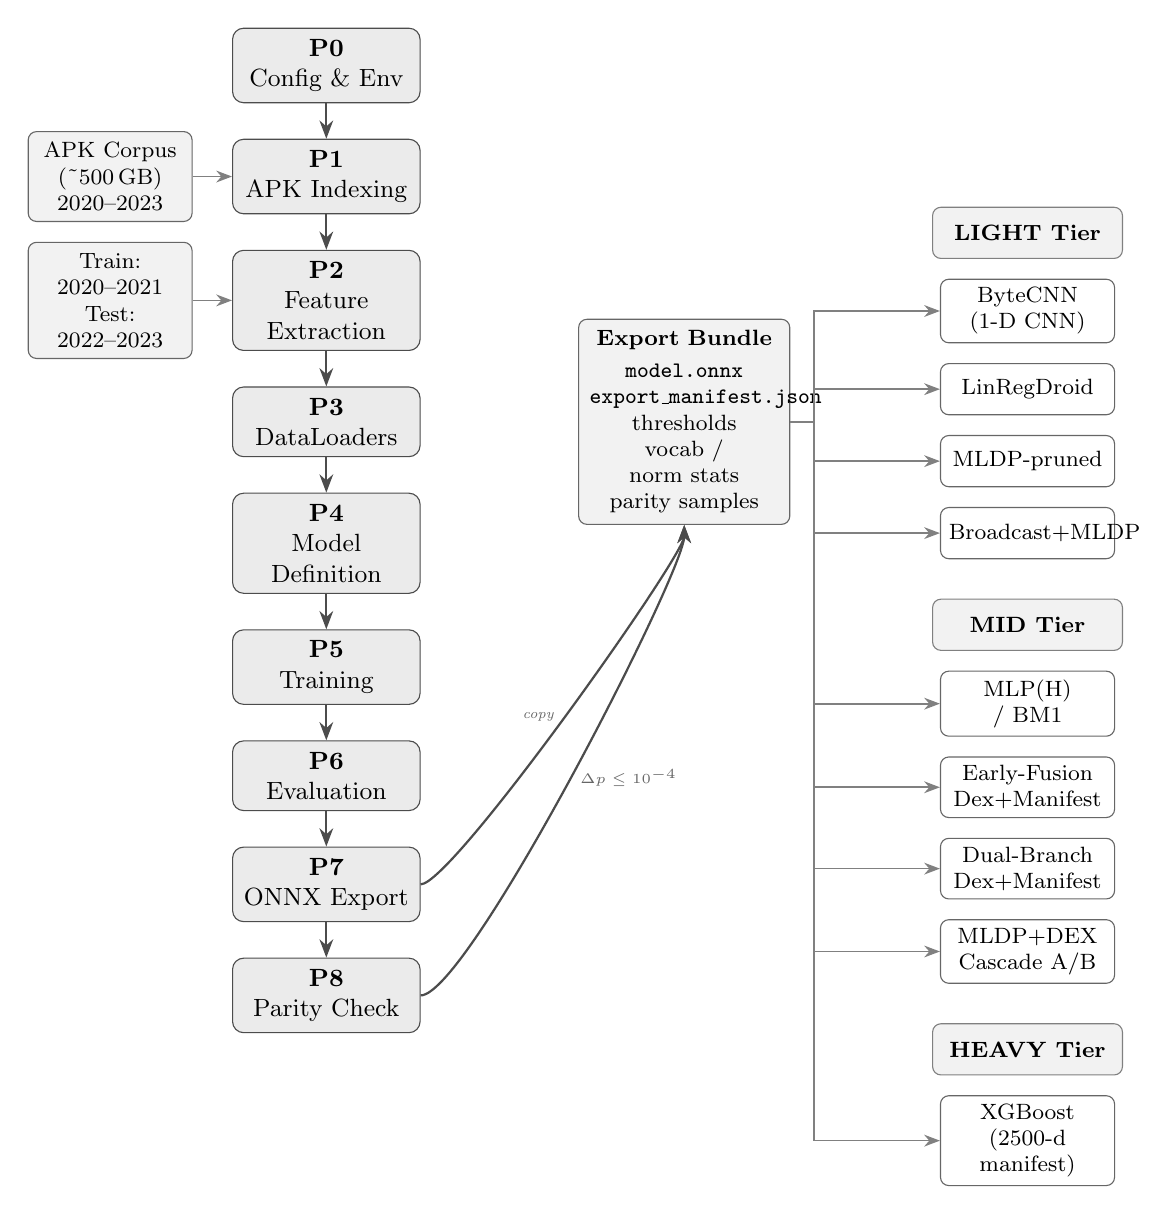
\begin{tikzpicture}[
				font=\small,
				>=Stealth,
				% Node styles
				phase/.style={
					rectangle, rounded corners=4pt,
					draw=black!70, fill=black!8,
					text width=2.1cm, align=center,
					minimum height=0.75cm, inner sep=4pt
				},
				model/.style={
					rectangle, rounded corners=3pt,
					draw=black!60, fill=white,
					text width=2.0cm, align=center,
					minimum height=0.65cm, inner sep=3pt,
					font=\footnotesize
				},
				tier/.style={
					rectangle, rounded corners=3pt,
					draw=black!50, fill=black!5,
					text width=2.2cm, align=center,
					minimum height=0.65cm, inner sep=3pt,
					font=\footnotesize\bfseries
				},
				decision/.style={
					diamond, aspect=2.2,
					draw=black!70, fill=black!10,
					text width=1.6cm, align=center,
					inner sep=2pt, font=\footnotesize
				},
				verdict/.style={
					rectangle, rounded corners=4pt,
					draw=black!80, fill=black!15,
					text width=1.8cm, align=center,
					minimum height=0.7cm, inner sep=4pt,
					font=\footnotesize\bfseries
				},
				output/.style={
					rectangle, rounded corners=3pt,
					draw=black!60, fill=black!5,
					text width=2.2cm, align=center,
					minimum height=0.65cm, inner sep=4pt,
					font=\footnotesize
				},
				arr/.style={->, thick, black!70},
				sarr/.style={->, semithick, black!50},
				label/.style={font=\tiny\itshape, black!60},
				groupbox/.style={
					draw=black!40, dashed, rounded corners=5pt,
					inner sep=6pt, fill=black!2
				}
				]
				
				%% ─── COLUMN 1: PC OFFLINE PIPELINE ───────────────────────────────────────
				\node[phase] (p0) at (0,0)     {\textbf{P0}\\Config \& Env};
				\node[phase, below=0.45cm of p0] (p1) {\textbf{P1}\\APK Indexing};
				\node[phase, below=0.45cm of p1] (p2) {\textbf{P2}\\Feature Extraction};
				\node[phase, below=0.45cm of p2] (p3) {\textbf{P3}\\DataLoaders};
				\node[phase, below=0.45cm of p3] (p4) {\textbf{P4}\\Model Definition};
				\node[phase, below=0.45cm of p4] (p5) {\textbf{P5}\\Training};
				\node[phase, below=0.45cm of p5] (p6) {\textbf{P6}\\Evaluation};
				\node[phase, below=0.45cm of p6] (p7) {\textbf{P7}\\ONNX Export};
				\node[phase, below=0.45cm of p7] (p8) {\textbf{P8}\\Parity Check};
				
				\draw[arr] (p0)--(p1); \draw[arr] (p1)--(p2); \draw[arr] (p2)--(p3);
				\draw[arr] (p3)--(p4); \draw[arr] (p4)--(p5); \draw[arr] (p5)--(p6);
				\draw[arr] (p6)--(p7); \draw[arr] (p7)--(p8);
				
				% Corpus note
				\node[output, left=0.5cm of p1, text width=1.8cm] (corpus)
				{APK Corpus\\(\textasciitilde500\,GB)\\2020--2023};
				\draw[sarr] (corpus) -- (p1);
				
				% Temporal split note
				\node[output, left=0.5cm of p2, text width=1.8cm] (split)
				{Train: 2020--2021\\Test: 2022--2023};
				\draw[sarr] (split) -- (p2);
				
				% Background box for PC pipeline
				%\begin{scope}[on background layer]
				% \node[groupbox, fit=(p0)(p1)(p2)(p3)(p4)(p5)(p6)(p7)(p8),
				%      label=above:{\normalsize\bfseries PC Offline Pipeline}] (pcbox) {};
				%\end{scope}
				
				%% ─── COLUMN 2: EXPORT BUNDLE ──────────────────────────────────────────────
				\node[output, right=2cm of p3, text width=2.4cm] (bundle) {
					\textbf{Export Bundle}\\[2pt]
					\texttt{model.onnx}\\
					\texttt{export\_manifest.json}\\
					thresholds\\
					vocab / norm stats\\
					parity samples
				};
				\draw[arr] (p7.east) .. controls +(0.4,0) and +(0,-0.4) .. (bundle.south) node[ midway,left, label]{copy} (bundle);
				\draw[arr] (p8.east) .. controls +(0.6,0) and +(0,-0.6) .. (bundle.south)
				node[midway, right, label]{$\Delta p \leq 10^{-4}$};
				
				%% ─── COLUMN 3: MODEL FAMILIES ─────────────────────────────────────────────
				\node[tier, right=1.8cm of bundle, yshift=2.4cm] (light)
				{LIGHT Tier};
				\node[model, below=0.25cm of light] (m1) {ByteCNN\\(1-D CNN)};
				\node[model, below=0.25cm of m1]   (m2) {LinRegDroid};
				\node[model, below=0.25cm of m2]   (m3) {MLDP-pruned};
				\node[model, below=0.25cm of m3]   (m4) {Broadcast+MLDP};
				
				\node[tier, below=0.5cm of m4] (mid) {MID Tier};
				\node[model, below=0.25cm of mid]  (m5) {MLP(H) / BM1};
				\node[model, below=0.25cm of m5]   (m6) {Early-Fusion\\Dex+Manifest};
				\node[model, below=0.25cm of m6]   (m7) {Dual-Branch\\Dex+Manifest};
				\node[model, below=0.25cm of m7]   (m8) {MLDP+DEX\\Cascade A/B};
				
				\node[tier, below=0.5cm of m8] (heavy) {HEAVY Tier};
				\node[model, below=0.25cm of heavy] (m9) {XGBoost\\(2500-d manifest)};
				
				\draw[sarr] (bundle.east) -- ++(0.3,0) |- (m1.west);
				\draw[sarr] (bundle.east) -- ++(0.3,0) |- (m2.west);
				\draw[sarr] (bundle.east) -- ++(0.3,0) |- (m3.west);
				\draw[sarr] (bundle.east) -- ++(0.3,0) |- (m4.west);
				\draw[sarr] (bundle.east) -- ++(0.3,0) |- (m5.west);
				\draw[sarr] (bundle.east) -- ++(0.3,0) |- (m6.west);
				\draw[sarr] (bundle.east) -- ++(0.3,0) |- (m7.west);
				\draw[sarr] (bundle.east) -- ++(0.3,0) |- (m8.west);
				\draw[sarr] (bundle.east) -- ++(0.3,0) |- (m9.west);
				
				
			\end{tikzpicture}%
		}
		
		\caption{Offline VigiDroid model-development pipeline. The PC-side workflow indexes APKs, extracts features, trains and exports ONNX bundles, and organizes the exported detectors into LIGHT, MID, and HEAVY inference tiers.}
		\label{fig:offline-workflow}
	\end{figure}
	
	\begin{figure}[H]
		\centering
		\resizebox{0.6\columnwidth}{!}{%
			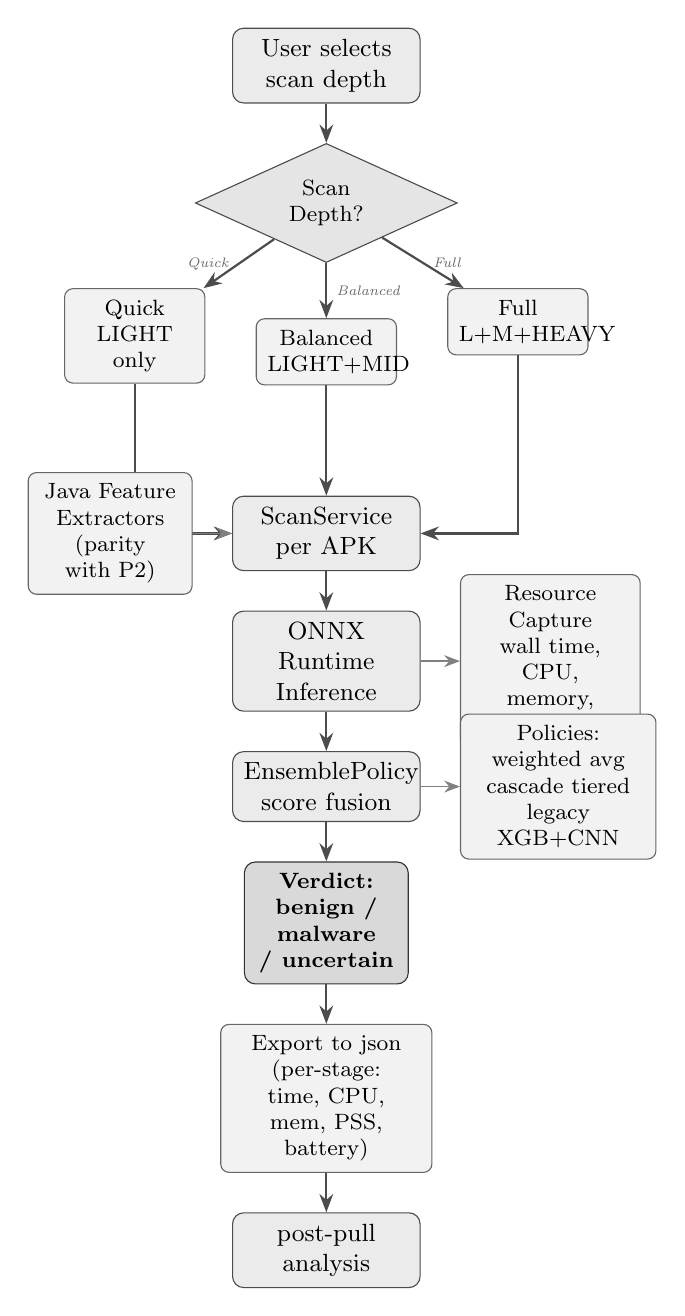
\begin{tikzpicture}[
				font=\small,
				>=Stealth,
				phase/.style={
					rectangle, rounded corners=4pt,
					draw=black!70, fill=black!8,
					text width=2.1cm, align=center,
					minimum height=0.75cm, inner sep=4pt
				},
				decision/.style={
					diamond, aspect=2.2,
					draw=black!70, fill=black!10,
					text width=1.6cm, align=center,
					inner sep=2pt, font=\footnotesize
				},
				verdict/.style={
					rectangle, rounded corners=4pt,
					draw=black!80, fill=black!15,
					text width=1.8cm, align=center,
					minimum height=0.7cm, inner sep=4pt,
					font=\footnotesize\bfseries
				},
				output/.style={
					rectangle, rounded corners=3pt,
					draw=black!60, fill=black!5,
					text width=2.2cm, align=center,
					minimum height=0.65cm, inner sep=4pt,
					font=\footnotesize
				},
				arr/.style={->, thick, black!70},
				sarr/.style={->, semithick, black!50},
				label/.style={font=\tiny\itshape, black!60},
				groupbox/.style={
					draw=black!40, dashed, rounded corners=5pt,
					inner sep=6pt, fill=black!2
				}
				]
				
				%% ─── VIGIDROID ON-DEVICE FLOW ────────────────────────────────────────────
				\node[phase] (ui) at (0,0) {User selects\\scan depth};
				\node[decision, below=0.5cm of ui] (depth) {Scan\\Depth?};
				
				\node[output, below left=0.7cm and 0.7cm of depth, text width=1.5cm] (dq)
				{Quick\\LIGHT only};
				\node[output, below=0.7cm of depth, text width=1.5cm] (db)
				{Balanced\\LIGHT+MID};
				\node[output, below right=0.7cm and 0.7cm of depth, text width=1.5cm] (df)
				{Full\\L+M+HEAVY};
				
				\draw[arr] (ui) -- (depth);
				\draw[arr] (depth) -- node[left, label]{Quick} (dq);
				\draw[arr] (depth) -- node[right, label]{Balanced} (db);
				\draw[arr] (depth) -- node[right, label]{Full} (df);
				
				\node[phase, below=1.4cm of db] (scan) {ScanService\\per APK};
				\draw[arr] (dq.south) |- (scan.west);
				\draw[arr] (db) -- (scan);
				\draw[arr] (df.south) |- (scan.east);
				
				\node[output, left=0.5cm of scan, text width=1.8cm] (java)
				{Java Feature\\Extractors\\(parity with P2)};
				\draw[sarr] (java) -- (scan);
				
				\node[phase, below=0.5cm of scan] (onnx) {ONNX Runtime\\Inference};
				\draw[arr] (scan) -- (onnx);
				
				\node[output, right=0.5cm of onnx, text width=2.0cm] (res)
				{Resource Capture\\wall time, CPU,\\memory, battery};
				\draw[sarr] (onnx) -- (res);
				
				\node[phase, below=0.5cm of onnx] (ens) {EnsemblePolicy\\score fusion};
				\draw[arr] (onnx) -- (ens);
				
				\node[output, right=0.5cm of ens, text width=2.2cm] (pol)
				{Policies:\\weighted avg\\cascade tiered\\legacy XGB+CNN};
				\draw[sarr] (ens) -- (pol);
				
				\node[verdict, below=0.5cm of ens] (verd) {Verdict:\\benign / malware\\/ uncertain};
				\draw[arr] (ens) -- (verd);
				
				\node[output, below=0.5cm of verd, text width=2.4cm] (json)
				%{\texttt{all\_scan\_metrics.json}\\
					{Export to json\\(per-stage: time, CPU,\\mem, PSS, battery)};
					\draw[arr] (verd) -- (json);
					
					\node[phase, below=0.5cm of json] (analyze)
					{%\texttt{analyze\_device\_scans.py}
						post-pull analysis};
					\draw[arr] (json) -- (analyze);
					
					
					
				\end{tikzpicture}%
			}
			
			\caption{VigiDroid on-device application flow. The app selects a scan depth, runs the corresponding model tiers through local feature extraction and ONNX Runtime inference, fuses model scores, reports a verdict, and writes resource metrics for post-device analysis.}
			\label{fig:vigidroid-app-flow}
		\end{figure}
		
		\FloatBarrier
		
		\section{Experiments}
		We evaluate each model on two axes: \textbf{offline quality} (accuracy, F1, ROC-AUC on temporal holdout APKs) and \textbf{on-device feasibility} (mean CPU, memory, battery, wall time per scan on a physical Android device).
		Tables~\ref{tab:offline-results} and~\ref{tab:device-results} split the planned comparison into offline quality and on-device feasibility metrics; values below are placeholders pending completed device campaigns and unified offline exports.
		Fig.~\ref{fig:inference time vs apk size} illustrates  (placeholder).
		
		\begin{table}[H]
			\caption{Planned offline quality comparison of thesis models (values TBD). Metrics are computed on the PC temporal test split.}
			\label{tab:offline-results}
			\centering
			\scriptsize
			\setlength{\tabcolsep}{3pt}
			\begin{tabular}{@{}l p{2.4cm} c c c@{}}
				\toprule
				\textbf{Model} & \textbf{Features} & \textbf{Acc.} & \textbf{F1} & \textbf{ROC-AUC} \\
				\midrule
				1-D CNN & Last 1024 APK bytes & -- & -- & -- \\
				LinRegDroid & Manifest permissions & -- & -- & -- \\
				MLDP-pruned & MLDP permissions & -- & -- & -- \\
				Broadcast+MLDP & Perms.+ receivers & -- & -- & -- \\
				MLP(H) / BM1 & DEX header & 0.966 & 0.944& 0.963 \\
				Early-Fusion Dex+Manifest & Header+ manifest BoW & -- & -- & -- \\
				Dual-Branch Dex+Manifest & Dual-branch fusion & -- & -- & -- \\
				MLDP+DEX cascade & MLDP $\parallel$ header & -- & -- & -- \\
				XGBoost & Multi-DEX manifest & -- & -- & -- \\
				%Ensemble (tiered) & Policy fusion & -- & -- & -- \\
				\bottomrule
			\end{tabular}
		\end{table}
		
		\begin{table}[H]
			\caption{Planned on-device feasibility comparison of thesis models (values TBD). Resource columns are derived from \texttt{all\_scan\_metrics.json}.}
			\label{tab:device-results}
			\centering
			\scriptsize
			\setlength{\tabcolsep}{3pt}
			\begin{tabular}{@{}l c c c c c@{}}
				\toprule
				\textbf{Model} & \textbf{CPU} & \textbf{Mem.} & \textbf{Batt.} & \textbf{Time} & \textbf{Feasible} \\
				\midrule
				1-D CNN & -- & -- & -- & -- & TBD \\
				LinRegDroid & -- & -- & -- & -- & TBD \\
				MLDP-pruned & -- & -- & -- & -- & TBD \\
				Broadcast+MLDP & -- & -- & -- & -- & TBD \\
				MLP(H) / BM1 & -- & -- & -- & -- & TBD \\
				Early-Fusion Dex+Manifest & -- & -- & -- & -- & TBD \\
				Dual-Branch Dex+Manifest & -- & -- & -- & -- & TBD \\
				MLDP+DEX cascade & -- & -- & -- & -- & TBD \\
				XGBoost & -- & -- & -- & -- & TBD \\
				%Ensemble (tiered) & -- & -- & -- & -- & TBD \\
				\bottomrule
			\end{tabular}
		\end{table}
		
		\begin{figure}[H]
			\centerline{\fbox{\parbox{0.92\linewidth}{\centering\vspace{2.8em}
						\textbf{[Figure 1 --- Placeholder]}\\
						Inference time vs apk size:\\
						UI $\rightarrow$ ScanService $\rightarrow$ tiered ONNX models $\rightarrow$ ensemble $\rightarrow$ metrics JSON\vspace{2.8em}}}}
			\caption{inference time vs apk size}
			\label{fig:inference time vs apk size}
		\end{figure}
		
		
		
		
		
		\begin{figure}[H]
			\centerline{\fbox{\parbox{0.92\linewidth}{\centering\vspace{2.8em}
						\textbf{[Figure 2 --- Placeholder]}\\
						Planned: accuracy vs.\ mean scan time (or Pareto plot)\\
						across models and scan levels\vspace{2.8em}}}}
			\caption{Planned trade-off figure: detection quality versus on-device cost across models and Quick/Balanced/Full scan depths. To be generated from offline + device metrics.}
			\label{fig:tradeoff}
		\end{figure}
		\textbf{Protocol (planned).}
		Labeled eval APKs (\texttt{eval\_XXXX\_benign/malware.apk}) on device; metrics pulled via ADB; offline labels from corpus year splits.
		
		
		\section{Conclusion}
		We described VigiDroid, a thesis framework for practical on-device Android malware pre-screening that unifies literature-based static detectors through a disciplined train-export-deploy pipeline and tiered ONNX orchestration on Android.
		By logging multi-dimensional resource metrics alongside fused verdicts, the system supports evidence-based selection of models that balance accuracy and mobile cost.
		Final quantitative results, ensemble calibration, and user-study implications will be reported once device experiments and figure generation are complete.
		
		\section*{Acknowledgment}
		The authors thank their supervisor and collaborators at the Department of Computer Science and Engineering, BUET, for guidance throughout this thesis.
		
		\begin{thebibliography}{00}
			\bibitem{bytecnn}
			C.~Hasegawa and H.~Iyatomi,
			``One-dimensional convolutional neural networks for Android malware detection,''
			in \textit{Proc.\ ICCE}, 2020.
			
			\bibitem{linregdroid}
			A.~Narayanan et al.,
			``LinRegDroid: Detection of Android malware using multiple linear regression,''
			\textit{Computers \& Security}, 2018.
			\bibitem{msdroid}
			Tao Peng et al.,
			``A Lightweight Multi-Source Fast Android Malware Detection Model,''
			\textit{Appl. Sci.}, 2022.
			
			
			\bibitem{broadcast}
			M.~Mohsen and A.~Ismail,
			``Detecting Android malwares by mining statically registered broadcast receivers,''
			\textit{Int.\ J.\ Advanced Computer Science and Applications}, 2017.
			\bibitem{seqmobile}
			Ruitao Feng et al.,
			``SeqMobile: An Efficient Sequence-Based Malware Detection System Using RNN on Mobile Devices''
			\textit{ 25th International Conference on Engineering of Complex Computer Systems (ICECCS)}, 2020.
			\bibitem{samadroid}
			Saba Arshad et al.,
			``SAMADroid: A Novel 3-Level Hybrid Malware Detection Model for Android Operating System''
			\textit{IEEE Access}, 2018.
			\bibitem{dldroid}
			Mohammed K. Alzaylaee et al.,
			``DL-Droid: Deep learning based android malware detection using real devices''
			\textit{IEEE Access}, 2020.
			
			\bibitem{mldp}
			S.~Wang et al.,
			``Permission extraction framework for Android malware detection,''
			\textit{IEEE Access}, 2019.
			
			\bibitem{msfdroid}
			Y.~Li et al.,
			``MSFDroid: Multi-stage fusion for Android malware detection,''
			\textit{IEEE Trans.\ Information Forensics and Security}, 2022.
			\bibitem{mh1m}
			Bragança, H., Kreutz, D., Rocha, V. et al. ,
			``MH-1M: A 1.34 Million-Sample Multi-Feature Android Malware Dataset with Rich Metadata.,''
			\textit{Sci Data 13, 153 . https://doi.org/10.1038/s41597-025-06469-5}, 2026.
			\bibitem{msfdroid}
			Tao Peng et al.,
			``A Lightweight Multi-Source Fast Android Malware Detection Model,''
			\textit{Appl. Sci.}, 2022.
			\bibitem{drebin}
			D.~Arp et al.,
			``Drebin: Effective and explainable detection of Android malware in your pocket,''
			in \textit{Proc.\ NDSS}, 2014.
			
			\bibitem{onnx}
			ONNX Runtime documentation,
			\url{https://onnxruntime.ai/}, accessed 2026.
		\end{thebibliography}
		
		
		
		
	\end{document}
